\section{Internet of Things}
\subsection{Vergangenheit, Gegenwart, Zukunft}
\begin{quote}
"`\textit{The most profound technologies are those that disappear}"' \\-- Mark Weiser, Chief Technologist at Xerox PARC \cite{weiser1991computer}
\end{quote}

1991 beschrieb M.Weiser in seinem einflussreichen Artikel \cite{weiser1991computer} eine Zukunft, in welcher der Computer komplett mit seiner Umgebung verschmilzt und somit unsichtbar für den Endnutzer wird. Dieses theoretische Paradigma wurde von ihm \ac{Ubicomp} -- die Omnipräsenz von Informationsverarbeitung -- getauft. Dieser Ansatz begründete sich auf den Erfolgen der \ac{GUI} als Interaktionsmodel über die, zu jener Zeit dominierende, textuelle Eingabe auf Konsolen-Basis. Eine \ac{GUI} stellt im Optimalfall eine Metapher zur physischen Welt dar (bspw. \textit{Computer Desktop} und reeller Schreibtisch). Nach \cite{weiser1991computer} wird es durch \ac{Ubicomp} möglich sein, diese Metaphern wieder zurückzuführen, d.h. die physische Welt wird durch die Verdrahtung mit seinen digitalen Repräsentanten wieder vereint. Das Ziel von \ac{Ubicomp} ist somit, die Einbettung des Computers in der physischen Welt, statt einer Manifestation der reellen Welt, innerhalb des Computers \cite{lyytinen2002ubiquitous}. 

Anfang der neunziger Jahre, war dieses Paradigma aufgrund fehlender Technologien nur schwer in die Realität umzusetzen. Kabellose Übertragung von Daten war weder standardisiert, noch technisch weit genug fortgeschritten, unzureichende Energiespeicher und die fehlende Rechenkapazität von Computern, waren nur einige Hindernisse, die zu diesem Zeitpunkt einer Verbreitung des \ac{Ubicomp} Paradigmas, außerhalb von wissenschaftlichen Experimenten im Weg stand \cite{lyytinen2002ubiquitous}.

Die Erfüllung zweier Regeln, haben sich für die Entwicklung der fehlenden Technologien als wichtig erwiesen: Komey's Law \cite{koomey2010law} und Moore's Law \cite{schaller1997moore}. Sie sagen voraus, dass alle 18 Monate sich der Preis pro Transistor halbiert und sich die Energieeffizienz gleichzeitig verdoppelt. Gut 30 Jahre nach der initialen Vision von \ac{Ubicomp} sind leistungsfähige Computer auf die Größe einer Streichholzschachtel geschrumpft, dauerhaft mit dem Internet verbunden und günstig. Durch diese stetige Verbesserung mobiler Hardware, das Durchsetzen von Kommunikationsprotokollen wie \textit{6LoWPAN} und die Motivation der Industrie, Prozesse immer weiter zu automatisieren (d.h. Industrie 4.0), hat sich das \acf{IoT} in seiner jetzigen Form entwickelt.

Der Begriff \ac{IoT} wurde 2002 in \cite{ashton2009internet} mit folgendem Zitat geschaffen:
\begin{quote}
    "`\textit{We need an internet for things, a standardized way for computers to understand the real world}"'
\end{quote}
 Hierbei bezog sich \cite{ashton2009internet} auf die RFID-Technologie, welche es erlaubt, reellen Objekten (engl. "`Things"') durch einen ID-Tag eine Identifikation und somit eine virtuelle Repräsentation zuzuweisen. RFID ist allerdings mehr als nur ein Barcode, denn es erlaubt Position und Status eines \textit{Things} in Echtzeit zu verfolgen \cite{atzori2010internet}. Dieses Erzeugen eines virtuellen Abbilds, gilt als Schlüssel-Technologie für das \ac{IoT}. Seit 2002 haben sich die zugrunde liegenden Technologien stetig weiterentwickelt und somit die Vision erweitert. \ac{IoT} hat sich zu einem der brisantesten Paradigmen des 21. Jahrhunderts entwickelt. Schon jetzt, existieren laut \cite{gartnerIoT} über 6.4 Milliarden \textit{Things} bzw. \textit{Smart Objects}, welche miteinander kommunizieren. Der anhaltende Trend zur Digitalisierung von Alltagsleben und Industrieprozessen durch \ac{IoT}, soll im Jahr 2020 die Anzahl von \textit{Smart Objects} auf über 21 Milliarden erhöhen. Zu diesem Zeitpunkt wird laut \cite{tan2010future} die Maschine-zu-Maschine (engl. "`\textit{thing-to-thing}"') Kommunikation, die der Mensch-zu-Mensch Kommunikation quantitativ übersteigen. Dieser Zuwachs an \textit{Things} und das einbinden neuer Technologien (bspw. Künstliche Intelligenz, siehe \cite{mehdi2017deeplearningIoT}) wird auch in Zukunft noch die Anforderungen und Visionen an \ac{IoT} formen \cite{Gubbi.2013}.
 
\subsection{Begriffsdefinition}
Das \acl{IoT} ist bestenfalls ein schwammig definierter Begriff. Es existiert keine breit angenommene Definition für \ac{IoT} \cite{atzori2010internet}. Dieses wird dadurch erschwert, dass durch die domänenübergreifende, organisatorische und technische Vielfalt innerhalb von \ac{IoT}-Systemen, sowie das breite Anwendungsspektrum von \ac{IoT} verschiedene Visionen für das Paradigma entstanden sind. \cite{atzori2010internet} hat diese Visionen in drei verschiedene Sichtweisen unterteilt: 

\paragraph{\textit{Things} orientiert} Hierbei handelt es sich um die originale Vision der Auto-ID labs, die von \cite{sarma2000networked} vorgestellt wurde:

\begin{quote}
    "`\textit{We envision a world in which all electronic devices are networked and every object, whether it is physical or electronic, is electronically tagged with information pertinent to that object.}"'
\end{quote}

Diese Vision von \ac{IoT} reflektiert die Anfänge des Begriffs, bei denen wenig Augenmerk auf Maschine-zu-Maschine Kommunikation gelegt wird. Vielmehr liegt der Fokus an dieser Stelle auf den \textit{Smart Objects}: Ihre Charakteristik (bspw. Identität, Verhalten, Intelligenz), Ausprägung (bspw. Sensor, Aktor, Transducer) und die genutzten Technologien (bspw. RFID, NFC, WISP).

\paragraph{Internet orientiert} In diesem Falle, wurde das Hauptaugenmerk der Vision auf die Kommunikation zwischen den einzelnen \textit{Smart Objects} gelegt. Aus dieser Sichtweise, definiert sich \ac{IoT} über die Standardisierung der Kommunikation, die Architektur und Orchestrierung von \ac{IoT}-Ökosystemen und die dafür notwendige Technologien (bspw. 6LoWPAN, MQTT). Das \ac{ITU} definiert seine Vision von \ac{IoT} in \cite{itut2012}, wie folgt: 

\begin{quote}
"`\textit{A global infrastructure for the Information Society, enabling advanced services by interconnecting (physical and virtual) things based on, existing and evolving, interoperable information and communication technologies}"'
\end{quote}

Diese Internet-zentrische Vision entspringt aus der Notwendigkeit, dass die schiere Masse an \textit{Things} neue Anforderungen, an die verwendete Technik stellt (bspw. Erweiterung des Adressraums duch IPv6). 

\paragraph{Semantik orientiert} Die auf Wissen basierenden Visionen zählen zu den neueren Perspektiven der \ac{IoT}. Der Schwerpunkt ist in diesem Fall nicht die Kommunikation und die beteiligten \textit{Smart Objects} sondern die Eigenschaften der ausgetauschten Daten, wie sie ausgetauscht, aufbereitet und gespeichert werden. In \cite{Kotis2012} und \cite{Singh2014} wird diese Vision beschrieben. Hierbei werden neue Herausforderungen wie die Interoperabilität von \textit{Smart Objects}, Sicherheit, Privatsphäre \cite{weber2010internet} und die Dringlichkeit neuer Speichertechnologien in den Vordergrund gestellt.

\begin{figure}[h]
    \centering
    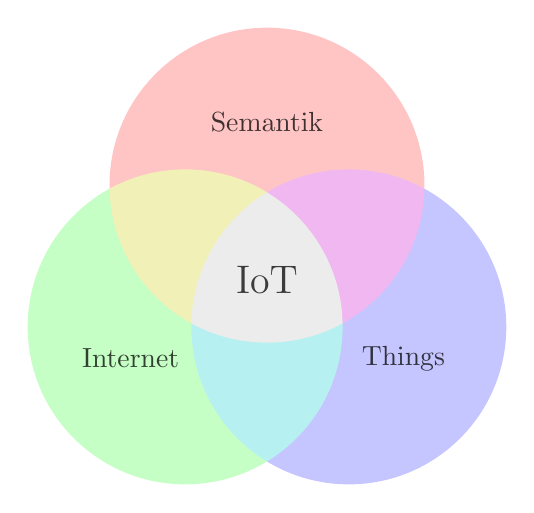
\begin{tikzpicture}[every path/.append style={fill opacity=0.75},]
      \begin{scope}[blend group = lighten]
        \fill[red!30!white]   ( 90:1.2) circle (2);
        \fill[green!30!white] (210:1.2) circle (2);
        \fill[blue!30!white]  (330:1.2) circle (2);
      \end{scope}
      \node at ( 90:2)    {Semantik};
      \node at ( 210:2)   {Internet};
      \node at ( 330:2)   {Things};
      \node [font=\Large] {\ac{IoT}};
    \end{tikzpicture}
    \caption{Das momentane Verständnis des \ac{IoT}-Begriffs stützt sich auf eine semantische, physische und kommunikative Sichtweise der Probleme. Darstellung angelehnt an \cite{atzori2010internet}}
    \label{fig:visions}
\end{figure}


Die vorgestellten Visionen (siehe Abbildung \ref{fig:visions}) reflektieren die Bestandteile eines \ac{IoT}-Systems aber auch die geschichtliche Herkunft des Paradigmas: von der Schaffung identifizierbarer \textit{Things} über der Kommunikation zwischen \textit{Smart Objects} zu der Semantik ausgetauschter Informationen. Es ist auch ersichtlich, dass das Verständnis von \ac{IoT} noch nicht komplett ausgereift ist \cite{atzori2010internet}. Deshalb ist es schwierig, eine allgemeingültige, auch in Zukunft treffende Definition, von \ac{IoT} zu formulieren. Mit dem Hinblick zu potentiellen Folgeparadigmen, wie das Internet of Everything \cite{Snyder2017}, ist es ohnehin fraglich, ob \ac{IoT} nur eine Zwischenstadium darstellt. Nichts desto trotz, wird für diese Thesis die in \cite{Misra2017} zu findende Definition verwendet: 
\begin{quote}
   "`\textit{The \ac{IoT}, a global network infrastructure, links uniquely identified physical and virtual objects, things and devices through the exploitation of data capture (sensing), communication and actuation capabilities. The underlying infrastructure of virtually represented \glq things \grq in an Internet-like structure includes existing and evolving Internet and network developments. Emerging services and applications will be characterised by a high degree of autonomous data capture, event transfer, network connectivity and interoperability.}"'
\end{quote}

Diese Definition vereint die vorherigen Visionen (\textit{Smart Objects}/\textit{Things}, Internet und Semantik) in einem treffenden Paragraph, ohne besonderes Augenmerk auf gewählten Technologien zu legen. Es wird ersichtlich, welche Objekte beteiligt sind, dass sie in einer Struktur verbunden werden müssen und autonom Daten austauschen müssen, um einen Mehrwert in Form von \textit{Services} darstellen zu können. 

\subsection{Charakterisierung von IoT}\label{subsec:characIot}
Wichtiger als die Definition von \ac{IoT} ist für diese Arbeit die Charakterisierung von \ac{IoT}. Hierbei werden die einzelnen Bestandteile von \ac{IoT}-Systemen definiert und ihr Zusammenspiel beschreiben. Wie der Begriff \acl{IoT} vermuten lässt, besteht er aus zwei Bestandteilen: \textbf{Internet} und \textbf{Things}.

\subsection{Things}
\textit{Things} ist der Oberbegriff für die physischen Objekte innerhalb einer \ac{IoT} Landschaft, die mit Umwelt und User interagieren. In diesem Zusammenhang sind zwei Begriffe von Bedeutung: \textbf{\ac{WSAN}} und \textbf{Smart Objects/connected Objects}.

\subsubsection{Smart Objects} \label{subsubsec:smartObjects}
\textit{Smart Objects} (auch \textit{Smart Devices}) stellen komplexe Interaktionsobjekte dar und sind auf der Komponentenebene die physikalischen Repräsentanten des Gesamtsystems. Ein \textit{Smart Object} kann aus ein oder mehreren Sensoren und Aktoren bestehen. \cite{Kortuem2010Smart} definiert \textit{Smart Objects} als ein dezentralisiertes System von lose gekoppelten, autonomen, physikalisch sowie digitalen identifizierbaren Objekten mit der Möglichkeit, ihre Umgebung durch Sensoren wahrzunehmen, diese Daten zu verarbeiten und über ein geteiltes Medium zu kommunizieren. \cite{mattern2010internet} beschreibt zusätzlich den Begriff der \textit{Effektorik}. Effektorik beschreibt die Fähigkeit von \textit{Smart Objects}, durch Aktoren (bspw. LED) digitale Signale in physikalische Signale (bspw. Bewegung durch Motoren oder visuelle Reize durch LEDs) zu transformieren. \cite{Kortuem2010Smart} beschreibt die grundsätzliche Charakteristiken von \textit{Smart Objects} wie folgt:
\begin{itemize}
    \item \textbf{Bewusstsein:} Ein \textit{Smart Object} ist in der Lage seine Umgebung und/oder das Verhalten des Nutzers wahrzunehmen und entsprechend der einprogrammierten Intelligenz (engl. "`Smartness"') darauf zu reagieren. \textit{Smartness} ist allerdings ein sehr dehnbarer Begriff. Es ist oftmals nicht künstliche Intelligenz gemeint, sondern schlichtweg das autonome Analysieren, Verarbeiten und Speichern von Daten. \textit{Smart Objects} besitzen ein Bewusstsein für \textbf{Ereignisse/Events} indem sie aperiodische, asynchrone Ereignisse (bspw. Temperaturschwankungen) analysieren oder auf Schritte in einem vordefinierten \textbf{Prozess} (bspw. Geschäftsprozess) reagieren. 
    \item \textbf{Darstellung:} Hierbei wird die Abstraktion der Logik, des \textit{Smart Objects} definiert. Unterschiedliche \textit{Smart Objects} können abhängig von ihrer Anwendung und der Komplexität ihrer Interaktion unterschiedlich gut geeignete für Programmiermodelle besitzen. \textbf{Aggregierende Funktionen} erlauben einem \textit{Smart Object} Daten aus Events zusammenzufassen, die dann vom Rest des Systems weiterverarbeitet werden. \textbf{Regeln} (bspw. "`Wenn \textit{Event x} dann \textit{Aktion y}"') erlauben es den \textit{Smart Devices} komplexere Logik darzustellen. Um auf Schritte innerhalb eines Prozesses angemessen zu reagieren, ermöglichen \textbf{Workflows} komplexe Prozesslogik abzubilden.
    \item \textbf{Interaktion:} Ein \textit{Smart Object} wird durch eine Reihe von Interaktionen charakterisiert, die es mit dem Nutzer und seiner Umgebung, durchführen kann. Ein \textit{Smart Object} kann \textbf{keine Interaktion} besitzen. Ein solches \textit{Smart Object} beschränkt sich auf die Aggregation von Daten. \textbf{Kontext-} und \textbf{Prozess-Interaktion} beziehen sich auf direkte Interaktionen mit dem Nutzer auf Basis von auditivem/visuellem/haptischem Feedback. Die Durchführung einer solchen Interaktion ist abhängig entweder vom Umgebungskontexts oder anhand eines Prozesschrittes, in dem sich das \textit{Smart Object} befindet.
\end{itemize}
Um \textit{Smart Objects} noch besser klassifizieren zu können, hat \cite{lopez2011taxonomy} das Modell "`I-S-A-D-N"' entworfen. Dieses Modell ordnet \textit{Smart Objects} anhand ihrer Fähigkeiten in verschiedene Klassen ein. Jeder Buchstabe in "`I-S-A-D-N"' steht für eine Fähigkeit von \textit{Smart Objects}  und kann beliebig kombiniert werden (siehe Tabelle \ref{tab:isadnKennz}). 
\begin{table}[h]
\centering
\begin{tabularx}{\textwidth}{llX}
\hline
\rowcolor[HTML]{EFEFEF} 
Kennz. & Bedeutung & Beschreibung \\ \hline
I      & Identität      & Das Objekt besitzt eine eindeutige Identität und die Möglichkeit Daten zu speichern. \\ \hline
S      & Sensorik       & Das Smart Object besitzt die Fähigkeit Daten aus seiner Umwelt zu erfassen. \\ \hline
A      & Aktorik        & Du Aktoren kann das \textit{Smart Object} seine Umwelt manipulieren. \\ \hline
D      & Determinierend & Das Objekt kann Entscheidungen auf Basis von programmierter Logik und von gesammelten Daten treffen. Diese Entscheidungen führen zu neuen physischen und digitalen Signalen. \\ \hline
N      & Netzwerkend   & Durch Einbindung in ein Netzwerk kann ein Objekt, bidirektional sich mit anderen \textit{Smart Objects} austauschen. \\ \hline                                                        
\end{tabularx}
\caption{Aspekte des "`I-S-A-D-N"'-Klassifikationsmodells für \textit{Smart Objects} nach \cite{lopez2011taxonomy} }
\label{tab:isadnKennz}
\end{table}

Abhängig der Komplexität des Anwendungsfalls können \textit{Smart Objects} verschiedene Kombinationen von Fähigkeiten besitzen. Ein ISN-Objekt ist ein \textit{Smart Object}, welches Identifizierbar ist, seine Umgebung bemisst und diese Daten speichert bzw. über das Netzwerk mit anderen Objekten kommuniziert. Als Einschränkung hierbei nennt \cite{lopez2011taxonomy}, dass ein \textit{Smart Device} mindestens IN-Fähigkeiten besitzt, also mindestens eine Identität besitzt und diese kommunizieren kann.

\subsubsection{\acl{WSAN}}\label{subsubsec:wsan}
\begin{figure}[h]
    \centering
    \includegraphics[width=0.75\textwidth]{bilder/chapter2/wsan.png}
    \caption{Ein typisches \ac{WSAN} nach \cite{feng2008wsan}. Zu sehen sind Aktor- und Sensorknoten, die in einem Netzwerk miteinander kommunizieren, welches von einer Basisstation aufgespannt wird}
    \label{fig:WSAN}
\end{figure}
\ac{WSAN} ist ein weiterer historisch und technisch wichtiger Baustein des \ac{IoT}-Ökosystems. Es beschreibt die Architektur und Module, welche durch kabellose Kommunikation sich in einem Netzwerk organisieren \cite{ferrara2013smart}. Die Abgrenzung von \ac{WSAN} zu \textit{Smart Objects} liegt darin, dass \ac{WSAN} sich weniger auf explizite Interaktionen mit dem User fokussieren, sondern sich vielmehr mit dem Erfassen und Erzeugen von Umgebungssignalen (bspw. Feuchtigkeit, Helligkeit, etc.) beschäftigen \cite{Madakam2015litRev}. \ac{WSAN}-Forschung ist dem \ac{IoT} vorangegangen. Der wissenschaftliche Fokus von \ac{WSAN}-Forschung liegt in der Reduktion von Energieverbrauch, physikalischer Größe, Vergrößerung von Senderadius und Verbesserung der Sensorik und Aktorik. Von dieser Entwicklung profitierte auch \ac{IoT} \cite{lopez2011taxonomy}.

\ac{WSAN} bestehen von einer Top-Level-Ansicht (siehe Abbildung \ref{fig:WSAN}) aus zwei Konstrukten: \textbf{Motes} (dt. "`Staubkorn"') und \textbf{Sinks} (dt. "`Senke"'). Diese Komponenten werden als \textbf{Nodes} (dt. "`Knoten"') bezeichnet und stellen die Knotenpunkte eines \acp{WSAN} dar. Sie bestehen aus autarken Embedded-Computern, welche entweder Sensoren oder Aktoren besitzen. Nodes mit Sensoren werden als Mote bezeichnet \cite{salarian2012coordination} und erfassen die physischen Signale der Umgebung. Sinks bezeichnen hierarchisch übergeordnete Knotenpunkte innerhalb eines \ac{WSAN}. Sinks besitzen Aktoren, die den Datenverkehr der Motes bündeln physischen Signale erzeugen.

Bei \ac{WSAN} als auch bei \textit{Smart Objects}, kristallisieren sich  \textbf{Sensoren} und \textbf{Aktoren} als fundamentale Bausteine heraus. 
\paragraph{Sensoren} Sie sind analog mit den fünf Sinnen des Menschen insofern, dass sie Computern erlauben, ihre Umgebung wahrzunehmen. Diese Wahrnehmung geschieht durch das Transformieren von (elektro-)magnetischer, akustischer und chemischer Signale in digitale und analoge Impulse. Diese Transformation von physikalischen Phänomenen in elektrische Signale macht jeden Sensor zu einem Transducer (engl. "`Wandler"'). 
\begin{figure}[h]
    \centering
    \includegraphics[width=0.75\textwidth]{bilder/chapter2/smartsensor.png}
    \caption{Als Smart-Sensor wird ein Sensor bezeichnet, der zusätzlich zu seinen Fähigkeiten als Transducer (physikal-zu-digital Wandler), die Signale in Ereignisse bzw. Datenpakete mit semantischer Bedeutung transformieren kann \cite{rayes2017internet}.}
    \label{fig:Smartsensor}
\end{figure}
Messungen, die ein Sensor nimmt, sind unbearbeitet und reflektieren die zugrunde liegenden Technik des Sensors (bspw. Schwankungen im Widerstand). Dieser "`rohe"' \textit{Output} ist nur schwer interpretierbar für Menschen. Erst eine Zuweisung der Rohdaten auf einen vorgegebenen Wertebereich gibt dem Output eine semantische Bedeutung. Dieser Vorgang ist in Abbildung \ref{fig:Smartsensor} illustriert. \cite{rayes2017internet} spricht hierbei von einem Smart-Sensor, da er eine programmierte Intelligenz besitzt, welche ein physikalisches Phänomen in ein semantisches Datenpaket umwandelt.

\begin{table}[h]
\centering
    \resizebox{\textwidth}{!}{
    \begin{tabular}{lllll}
    \hline
    \rowcolor[HTML]{EFEFEF} 
    Physikalisches Signal & Beispiel          & Output                  & Output-Format  & Einheit \\ \hline
    (Elektro)Magnetisch   & Erdmagnetfeld     & Himmelsrichtung         & $[0;360] $     & Grad    \\ \hline
    Chemisch              & $CO_{2}$-Sensor  & $CO_{2}$-Konzentration & $[0;100]$      & PPM     \\ \hline
    Akustisch             & Ultraschallsensor & Distanz                 & $[10;120]$     & cm      \\ \hline
    Position              & GPS               & Koordinaten             & $([-90;+90],[-180; 180])$  & (Längengr., Breitengr.) \\  \hline
    Photoelektrisch       & Bewegungsmelder   & Bewegung                & ${True,False}$ & Boolean \\  \hline
    \end{tabular}
    }
\caption{Sensortypen und beispielhafte Vertreter. Obwohl sämtliche Sensoren analoge bzw. digitale Daten schicken, Sensoren können stark unterschiedliche Outputs besitzen. Tabelle angelehnt an \cite{lopez2011taxonomy}}
\label{tab:sensorbsps}
\end{table}

In Tabelle \ref{tab:sensorbsps} gibt es eine Aufstellung von Sensor-Typen, sowie Beispiele aus der jeweiligen Klasse. Wichtig ist hierbei anzumerken, dass es für fast jegliche Art von erfassbaren Phänomenen, mehrere alternative Sensortechnologien existieren. Ausschlaggebend können hierbei Kriterien wie die Kosten, Reaktionszeit, Genauigkeit und Formfaktors des Sensors sein. Auch die Umgebung selbst kann ausschlaggebend für den Sensor-Typ sein.

\paragraph{Aktoren} stellen Wandler oder "`\textit{Transducer}"' dar, welche digitale Signale in physikalische Phänomene umwandeln. Diese Aktionen ermöglichen es, einem \ac{IoT}-System seine Umwelt zu manipulieren und auf Interaktionen mit dem Nutzer zu reagieren. 

\begin{table}[H]
\centering
\resizebox{\textwidth}{!}{
    \begin{tabular}{lllll}
    \hline
    \rowcolor[HTML]{EFEFEF} 
    Physikalische Aktion  & Beispiel           & Output-Typ  & Wertebereich    & Einheit         \\ \hline
    Visuell               & RGB LED            & Lichtimpuls & $[0;360]$       & RGB-Wert        \\ \hline
    Bewegung              & elektrischer Motor & Rotation    & $[-100;100]$ & Geschwindigkeit    \\ \hline
    Akustisch             & Lautsprecher       & Geräusch    & $[10;120]$      & Dezibel         \\ \hline
    \end{tabular}}
\caption{Typen von Aktoren}
\label{tab:typesOfActutors}
\end{table}

Die Definition von Aktor ist unterschiedlich, während eine Anzahl von Quellen auf die traditionelle Definition von Aktor ("`Umwandeln von elektrischem Signal in mechanische Bewegung"') bevorzugen, wird im \ac{IoT}-Kontext auch oft Transducer, welche Visuelle/Elektromagnetische Phänomene erzeugen als Aktoren bezeichnet \cite{Dunko2006reference}. Da ein Relais, welches mechanisch eine Ampel steuert \cite{salarian2012coordination}, als Aktor im traditionellen Sinn gilt, ist auch schlüssig einen Knoten, welcher digital eine LED ansteuert, auch als Aktor zu bezeichnen. Aus diesem Grund wird die \ac{IoT}-zentrische Verständnis von Aktoren für den Rest der Thesis verwendet. In Tabelle \ref{tab:typesOfActutors} wird eine Liste mit Beispielen von Aktor-Typen gezeigt. 

\subsection{Internet}
Kommunikation, Orchestrierung und Interoperabilität zwischen \textit{Things} ist die zweite Säule des \acp{IoT}. Ähnlich wie bei der Definition von \textit{Things}, existiert auch hier keine breit angenommene Begriffserklärung und verwendete Technologien. Die Kommunikation zwischen \textit{Things} ist facettenreich und und kann von verschiedenen Blickwinkeln betrachtet werden: Der verwendeten Technologien, der Organisationsstruktur oder der Semantik (bspw. Interoperabilitäts-Protokolle). Da sich diese Arbeit u.\,a. damit auseinandersetzt, treffende Metaphern für die Domäne der \ac{IoT} zu finden, ist organisatorische bzw. architekturelle Aspekt der Interessanteste.
\begin{figure}[h]
    \centering
    \includegraphics[width=0.85\textwidth]{bilder/chapter2/iotlayers.png}
    \caption{Schichtenmodell von einer typischen \ac{IoT} Infrastruktur nach \cite{bandyopadhyay2011internet}}
    \label{fig:iotlayer}
\end{figure}
Eine abstrahierte Version der \ac{IoT}-Architektur, welche wenig Wert auf verwendete Technologien legt, ist in Abbildung \ref{fig:iotlayer} zu sehen. Laut \cite{bandyopadhyay2011internet} besteht eine solche Architektur aus sechs Schichten. Die unteren drei Schichten setzen sich direkt mit dem Erheben und dem Transport von Daten auseinandersetzen. Diese Schichten befinden sich nah an der Grenze zur physikalischen Welt und werden deshalb als Edge-Layer bezeichnet. Die oberen Schichten beschäftigen sich mit der Transformation und Filterung der Daten, in einer Form, dass sie von Endnutzer-Applikationen verwendet werden können.  

\paragraph{Edge-Schicht} Sie wurde in den vorherigen Kapitel schon beschrieben. Es handelt sich hierbei um die konkreten Physikalischen Ressourcen: Sensoren und Aktoren bzw. \textit{Smart Objects}. Alle Objekte auf dieser Ebene sind eindeutig Identifizierbar (bspw. via RFID), besitzen die Möglichkeit physikalische Signale in elektrische umzuwandeln (bzw. umgekehrt) und per Kommunikationsmedium (bspw. WiFi oder Bluetooth) mit der darüberliegenden Schicht zu teilen.

\paragraph{Access-Gateway-Schicht} Diese Schicht verbindet die Objekte der Edge-Schicht, bündelt die im \ac{IoT}-System erzeugten Daten und verschickt diese an die weiterverarbeitenden Schnittstellen. Auch das \textit{Monitoring} von Objekten und Datensicherheit spielt auf dieser Ebene eine tragende Rolle. 

\paragraph{Internet-Schicht} Diese Ebene symbolisiert das unterliegende Kommunikationsmedium, das Internet. Daten, die sich an der Gateway-Schichte sammeln, werden über das Internet versendet. Diese Schicht beherbergt den Transport Layer des OSI-Modells inklusive UDP/TCP/IP-Stack und HTTP.

\paragraph{Middleware-Schicht} Sie ist die erste reine Software-Schicht. Die Middleware bildet das softwareseitige Herzstück des \ac{IoT}-Stacks und befasst sich damit, den bidirektionalen Austausch von Daten zu ermöglichen und den softwareseitigen Zugriff auf das \ac{IoT} System zu verwalten. Hierfür hat sich das \ac{SOA} Paradigma in der Vergangenheit für wegweisend erwiesen \cite{laliwala2008event}. Auf dieser Schicht befindet sich die Logik, die durch das \ac{EUD}-Werkzeug erzeugt wird.
\begin{figure}[h]
    \centering
    \includegraphics[width=0.85\textwidth]{bilder/chapter2/iotsoa.png}
    \caption{IoT Middleware-Schicht als \ac{SOA} nach \cite{bandyopadhyay2011internet}}
    \label{fig:iotsoa}
\end{figure}
Wie in Abbildung \ref{fig:iotsoa} zu sehen ist, abstrahiert die Middleware heterogene \textit{Smart Objects} bzw. Nodes in adressierbare, eindeutig identifizierbare, virtuelle Ressourcen (\textit{Object Abstraction}). Die Middleware kapselt einzelne oder mehrere Ressourcen zu Services mit wohl definierten Schnittstellen zusammen, um die Verwaltung und Nutzbarkeit der Objekte zu verbessern (\textit{Service Management}). Zu guter Letzt lassen sich einzelne Services zu Workflows, welche eine Businesslogik abbilden kompositionieren (\textit{Service Composition}). Durch dieses \ac{SOA}-Modell erlaubt es die Middleware, viele heterogene Ressourcen miteinander zu vereinigen und sie der Applikationslogik bereitzustellen. 

Die \textbf{Kommunikation} zwischen den (virtuellen) Ressourcen bzw. den Services wird als aperiodisch, parallel und Event-basiert charakterisiert (\cite{serpanos2018iot}, \cite{laliwala2008event}, \cite{lan2014event}). Laut \cite{serpanos2018iot} wird die Signalverarbeitung in traditionell geschlossenen System, in periodischen Zyklen ausgewertet. Dies ist in \ac{IoT}-Systemen aufgrund räumlicher Verteilung von Nodes und der gestiegene Energiebedarf durch kabellose Datenübertragung nicht praktikabel. Aus diesen Gründen, muss davon ausgegangen werden, dass Nodes ihre Daten in \textbf{aperiodischen} Zyklen zusenden. Des Weiteren wird durch die verteilte Kommunikation innerhalb eines \ac{IoT}-Systems, es als parallel und asynchron charakterisiert. Hierbei stellen \textit{Events} laut \cite{serpanos2018iot} einen zentralen Baustein dar. Events (dt. "`Ereignisse"') werden von Nodes erzeugt und/oder konsumiert. Events werden durch ein \textit{key-value pair} oder aufgrund ihrer Lebenszeit und temporalen Verarbeitung als \textit{time-value pair} beschrieben. Das key-value pair wird laut \cite{serpanos2018iot} durch ein fünffach Tupel beschrieben:
\begin{equation}
    \left \langle key, payload, sender, receiver, timestamp \right \rangle
\end{equation}
Diese Events werden zwischen den Nodes über definierte Kommunikationskanäle, sogenannte \textit{Links}, versendet. Ankommende Events werden von den Nodes reaktiv verarbeitet.

\subsection{cBlocks}
\acp{cBlock} ist ein \textit{Prototyping}-Werkzeug das im Zuge des \textit{PROFI}-Projekts von \cite{weckbach2018cblocks} entwickelt wurde. Es erlaubt Nutzern funktionale \ac{IoT}-Prototypen zu bauen, ohne Expertise in Elektrotechnik oder \textit{Embedded Software} zu besitzen.

Bei \acp{cBlock} werden einzelne Aktoren und Sensoren wie in einem \acp{WSAN} in Knoten gekapselt. Jeder Knoten stellt ein \ac{cBlock} (siehe Abbildung \ref{fig:cblockfoto}) dar, der entweder in Form eines Sensors Events/Ereignisse erfasst oder in Form eines Aktors Events/Ereignisse erzeugt. 

Der Nutzer (bspw. Designer) kann ISN-, IAN- und ISAN-\textit{Smart Objects}-Prototypen mit \acp{cBlock} erstellen. Hierfür werden \acp{cBlock} mit einer Basisstation kabellos verbunden und nach einem Pairing-Vorgang in das Netzwerk eingegliedert \cite{serdarusic2018pairing}. Der Verbund von Knoten stellt dann ein virtuelles \textit{Smart Object} dar.

\acp{cBlock} besitzt zum Zeitpunkt des Verfassens dieser Thesis (Aug. 2018) keine Möglichkeit für Laien Programmlogik zu implementieren. Lediglich eine \textit{Visualizer}-\acs{GUI} erlaubt es dem Endnutzer die erfassten und erzeugten Daten zu visualisieren. \acp{cBlock} besitzt somit keine Möglichkeit für Laien D-\textit{Smart Objects} (siehe Tabelle \ref{tab:isadnKennz}) zu erstellen, die Kontext- und Prozessinteraktionen erlauben. Dies ist wie schon in der Einleitung geschrieben (siehe Kapitel \ref{sec:1_kontext}), der Ansatzpunkt für das \ac{EUD}-Konzept.

\subsubsection*{Zusammenfassung}
In diesem Kapitel wurden die grundlegenden Züge von \ac{IoT} charakterisiert, die für diese Arbeit relevant sind. Der \ac{IoT}-Begriff umschließt die Kommunikation zwischen verteilten, digital identifizierbaren Objekten. Diese Objekte (\textit{Smart Objects}) unterschiedlicher Komplexität, erreichen es durch Datensammlung, Datenverarbeitung und physikalische Manipulation ihre Umwelt wahrnehmen bzw. in sie einzugreifen. Wahrnehmung und Manipulation wird durch die Verwendung von \textbf{Sensoren} und \textbf{Aktoren} erreicht. In einem Netzwerk solcher Objekte (d.\,h. Nodes), geschieht Kommunikation über ein geteiltes Medium (bspw. WiFi) und in weiter verteilten Systemen über das Internet. Nodes kommunizieren anhand von Events parallel und in aperiodischen Zyklen miteinander. Diese Events werden transformiert und enden in Aktionen, wie das Speichern/Präsentieren von Daten oder Interaktionen mit der Umwelt und dem Endnutzer. \acp{cBlocks} stellt sich hierbei als ein Werkzeug dar, das die technische Komplexität der Elektrotechnik und \textit{Embedded-Software} für domänenfremden Endnutzern weg zu abstrahiert.

Ziel von \ac{IoT} ist es, durch die Verschmelzung digitaler und reeller Welt, reichhaltigere Benutzerinteraktionen zu ermöglichen.